\section{Bode-Diagramm}

Das Bode-Diagramm ist eine weitere Variante, den Frequenzgang $G(j \omega)$ grafisch darzustellen.
Die Darstellung beinhaltet zwei Graphen.

\begin{itemize}
    \item Amplitudengang $|G(j \omega)|$ in Dezibel $\deci \bel$
    \item Phasengang $\angle G(j \omega)$ in Grad $\degree$
    \item Die Frequenzachse ist \textbf{logarithmisch} mit $\log_{10}(\omega)$
\end{itemize}


% Bei zu wenig Platz weglassen
\subsubsection{Logarithmische Frequenzachse}

\begin{itemize}
    \item Serieschaltung von Systemen
        $$ G(j \omega) = G_1(j \omega) \cdot G_2(j \omega) $$

    \begin{itemize}
        \item Amplitudengang
            $$ |G(j \omega)| = |G_1(j \omega)| \cdot |G_2(j \omega)| $$
            $$ |G(j \omega)|_{\deci \bel} = |G_1(j \omega)|_{\deci \bel} + |G_2(j \omega)|_{\deci \bel} $$
            \textrightarrow\ Grafisch multiplizieren wäre schwierig, grafisch addieren geht gut
    \end{itemize}

    \begin{itemize}
        \item Amplitudengang
            $$ \angle G(j \omega) = \angle G_1(j \omega) +  \angle G_2(j \omega) $$
            \textrightarrow\ Die Phase muss nicht logarithmisch sein, wir haben schon eine Addition 
    \end{itemize}
\end{itemize}


\subsection{Vorgehen: Bode-Diagramm zeichnen}

Das Diagramm wird approximativ mit \textbf{Geraden} gezeichnet!

\begin{itemize}
    \item Frequenzgang in folgende Form bringen:
        $$ G(j \omega) = K_0 \cdot (j \omega)^v \cdot \frac{(1 + T_{n0} \cdot j \omega)\cdot (1 + T_{n1} \cdot j \omega) \cdot \ldots}
        {(1 + T_{p0} \cdot j \omega)\cdot (1 + T_{p1} \cdot j \omega) \cdot \ldots} \cdot e^{- j \omega T_t} $$
    \begin{itemize}
        \item Für $\omega = 0$ sind alle $(1 + T \cdot j \omega) = 1 = 0 \, \deci \bel$
        \item Für $\omega = \frac{1}{T}$ sind alle  $(1 + T \cdot j \omega) = 1 + j = \sqrt{2} \cdot e^{j \frac{\pi}{4}} 
            = 3 \, \deci \bel \angle 45 \, \degree$
    \end{itemize}
    \item Frequenzen der Nullstellen berechnen: $\omega = \frac{1}{T_n}$
    \item Frequenzen der Polstellen berechnen: $\omega = \frac{1}{T_p}$


    \item Jede \textbf{Nullstelle} bewirkt
    \begin{itemize}
        \item einen Knick um $+ 20 \deci \bel$ / Dekade \textbf{nach oben} im Amplitudengang
        \item Einen Phasenhub von $+ 90 \, \degree$ \textrightarrow\ $+ 45 \, \degree$ beim Knick
    \end{itemize}
    \item Jede \textbf{Polstelle} bewirkt
    \begin{itemize}
        \item einen Knick um $- 20 \deci \bel$ / Dekade \textbf{nach unten} im Amplitudengang
        \item Einen Phasenverlust von $- 90 \, \degree$ \textrightarrow\ $- 45 \, \degree$ beim Knick
    \end{itemize}
    \item Einzelne Faktoren einzeichnen
    \item Grafische Addition der Faktoren für gesamten Frequenzgang
\end{itemize}


\example{Bode-Diagramm zeichnen}


%\begin{center}
    % Gain
    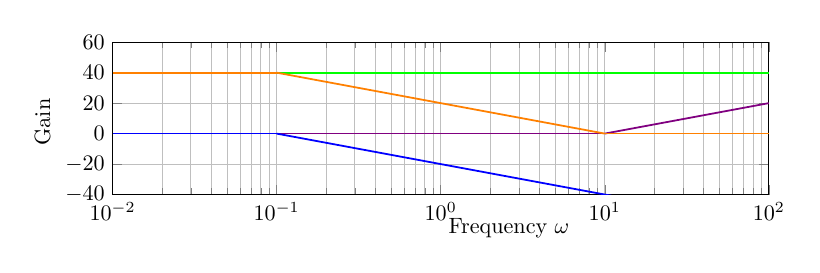
\begin{tikzpicture}
        [
            scale = 0.8,
            >=latex
        ]
        \begin{axis}
            [
                width=12cm,
                height=4cm,
                xmode=log,
                xmin=0.01, xmax=100, ymin=-40, ymax=60,
                x label style={anchor=west},
                xlabel=Frequency $\omega$,
                y label style={anchor=south},
                ylabel=Gain $\deci \bel$,
                xmajorgrids=true,
                xminorgrids=true,
                ymajorgrids=true
            ]
            
            % K_0
            \addplot[thick, color=green, domain=0.01:100]{40};

            % Nullstelle
            \addplot[thick, color=violet, domain=0.01:10]{0};               % start bis Knick
            \addplot[thick, color=violet, domain=10:100]{20*log10(x)-20};   % ab Knick nach oben    

            % Polstelle
            \addplot[thick, color=blue, domain=0.01:0.1]{0};                % start bis Knick
            \addplot[thick, color=blue, domain=0.1:100]{-20*log10(x)-20};   % ab Knick nach oben    
            
            % Grafische Addition
            \addplot[thick, color=orange, domain=0.01:0.1]{40};    
            \addplot[thick, color=orange, domain=0.1:10]{-20*log10(x)+20};        
            \addplot[thick, color=orange, domain=10:100]{0};      
           
        \end{axis}
        
    \end{tikzpicture}

    \vspace{0.3cm}


    % Phase
    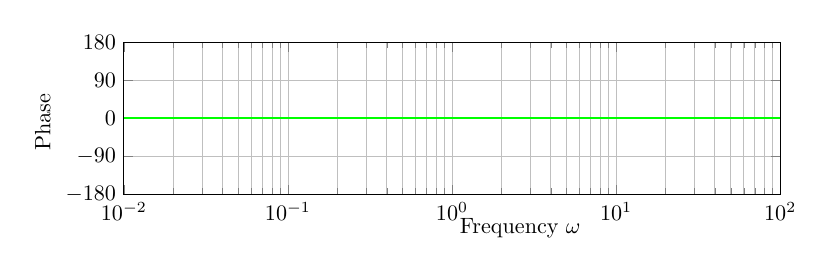
\begin{tikzpicture}
        [
            scale = 0.8,
            >=latex
        ]
        \begin{axis}
            [
                width=12cm,
                height=4cm,
                xmode=log,
                xmin=0.01, xmax=100, ymin=-180, ymax=180,
                x label style={anchor=west},
                xlabel=Frequency $\omega$,
                y label style={anchor=south},
                ylabel=Phase $\degree$,
                ytick={-180, -90, 0, 90, 180},
                % yticklabels={-180, -90, 0, 90, 180},
                xmajorgrids=true,
                xminorgrids=true,
                ymajorgrids=true
            ]
            
            % K_0
            \addplot[thick, color=green, domain=0.01:100]{0};
                
            % Nullstelle
            % \addplot[thick, color=violet, domain=0.01:1]{0};              % start bis Knick
            % \addplot[thick, color=violet, domain=1:10]{};        % ab Knick nach oben    
            
            % Polstelle
            % \addplot[thick, color=blue, domain=0.01:0.1]{0};                % start bis Knick
            % \addplot[thick, color=blue, domain=0.1:100]{-20*log10(x)-20};   % ab Knick nach oben    
            
            % Grafische Addition
            % \addplot[thick, color=orange, domain=0.01:0.1]{40};    
            % \addplot[thick, color=orange, domain=0.1:10]{-20*log10(x)+20};        
            % \addplot[thick, color=orange, domain=10:100]{0};      


            
        \end{axis}
            
    \end{tikzpicture}
\end{center}